\documentclass[a4paper,12pt]{article}

\usepackage[margin=0.8in]{geometry} % Sets a 0.8 inch margin on all four sides 
\usepackage{parskip} % Block Paragraphs
\usepackage{fancyhdr} % Fancy headers and footers
\usepackage{graphicx} % Enables images
\usepackage{pdfpages} % Embedded PDF files
\usepackage{caption} % Enables captions
\usepackage{mdframed} % Enables frames
\usepackage{verbatim} % Enables insertion of text files
\usepackage{wrapfig} % Wrapped figures
\usepackage{algorithm2e} % Algorithms
\usepackage{verbatim} % Embed text files
\usepackage[colorlinks=true,urlcolor=blue,linkcolor=blue,linktocpage=true]{hyperref} % Hypertext referencing

\usepackage{enumitem}
\newlist{arrowlist}{itemize}{1}
\setlist[arrowlist]{label=$\Rightarrow$} % Use command \begin {arrowlist} rather than \begin{itemize} for arrows

\usepackage{color} % Enables colours
\definecolor{darkpurple}{rgb}{0.4, 0.0, 0.4} % Defines a dark purple colour
\definecolor{javared}{rgb}{0.6,0,0} % for strings
\definecolor{javagreen}{rgb}{0.25,0.5,0.35} % comments
\definecolor{javapurple}{rgb}{0.5,0,0.35} % keywords
\definecolor{javadocblue}{rgb}{0.25,0.35,0.75} % javadoc

\pagestyle{fancy} % Set new page style
\frenchspacing % One space after a full stop
\parindent=0in % Do not indent paragraphs
\brokenpenalty10000\relax % Do not page break at a hyphen

\fancyhf{} % clear all header and footers
\renewcommand{\headrulewidth}{0pt} % remove the header rule
\rfoot{\thepage} 

\usepackage{listings}
  \usepackage{courier}
  \lstloadlanguages{C++}
  \lstset{
         language=C++,
         basicstyle=\footnotesize\ttfamily, 
         numbers=left,               
         numberstyle=\tiny,          
         numbersep=10pt,              
         tabsize=4,                  
         extendedchars=true,         
         breaklines=true,            
    	 frame=lrtb,         
         keywordstyle=\color{javapurple}\bfseries,
         stringstyle=\color{javared},
         commentstyle=\color{javagreen},
         morecomment=[s][\color{javadocblue}]{/**}{*/},
         showspaces=false,           
         showtabs=false,            
         xleftmargin=17pt,
         framexleftmargin=17pt,
         framexrightmargin=5pt,
         framexbottommargin=4pt,
         %backgroundcolor=\color{},
         showstringspaces=false      
 }

\DeclareCaptionFont{white}{\color{white}}
\DeclareCaptionFormat{listing}{\colorbox[cmyk]{0.43, 0.35, 0.35,0.01}{\parbox{\textwidth}{\hspace{15pt}#1#2#3}}}
\captionsetup[lstlisting]{format=listing,labelfont=white,textfont=white, singlelinecheck=false, margin=0pt, font={bf,footnotesize}}

\begin{document}

\includepdf{title/title_page.pdf} % Include title page
%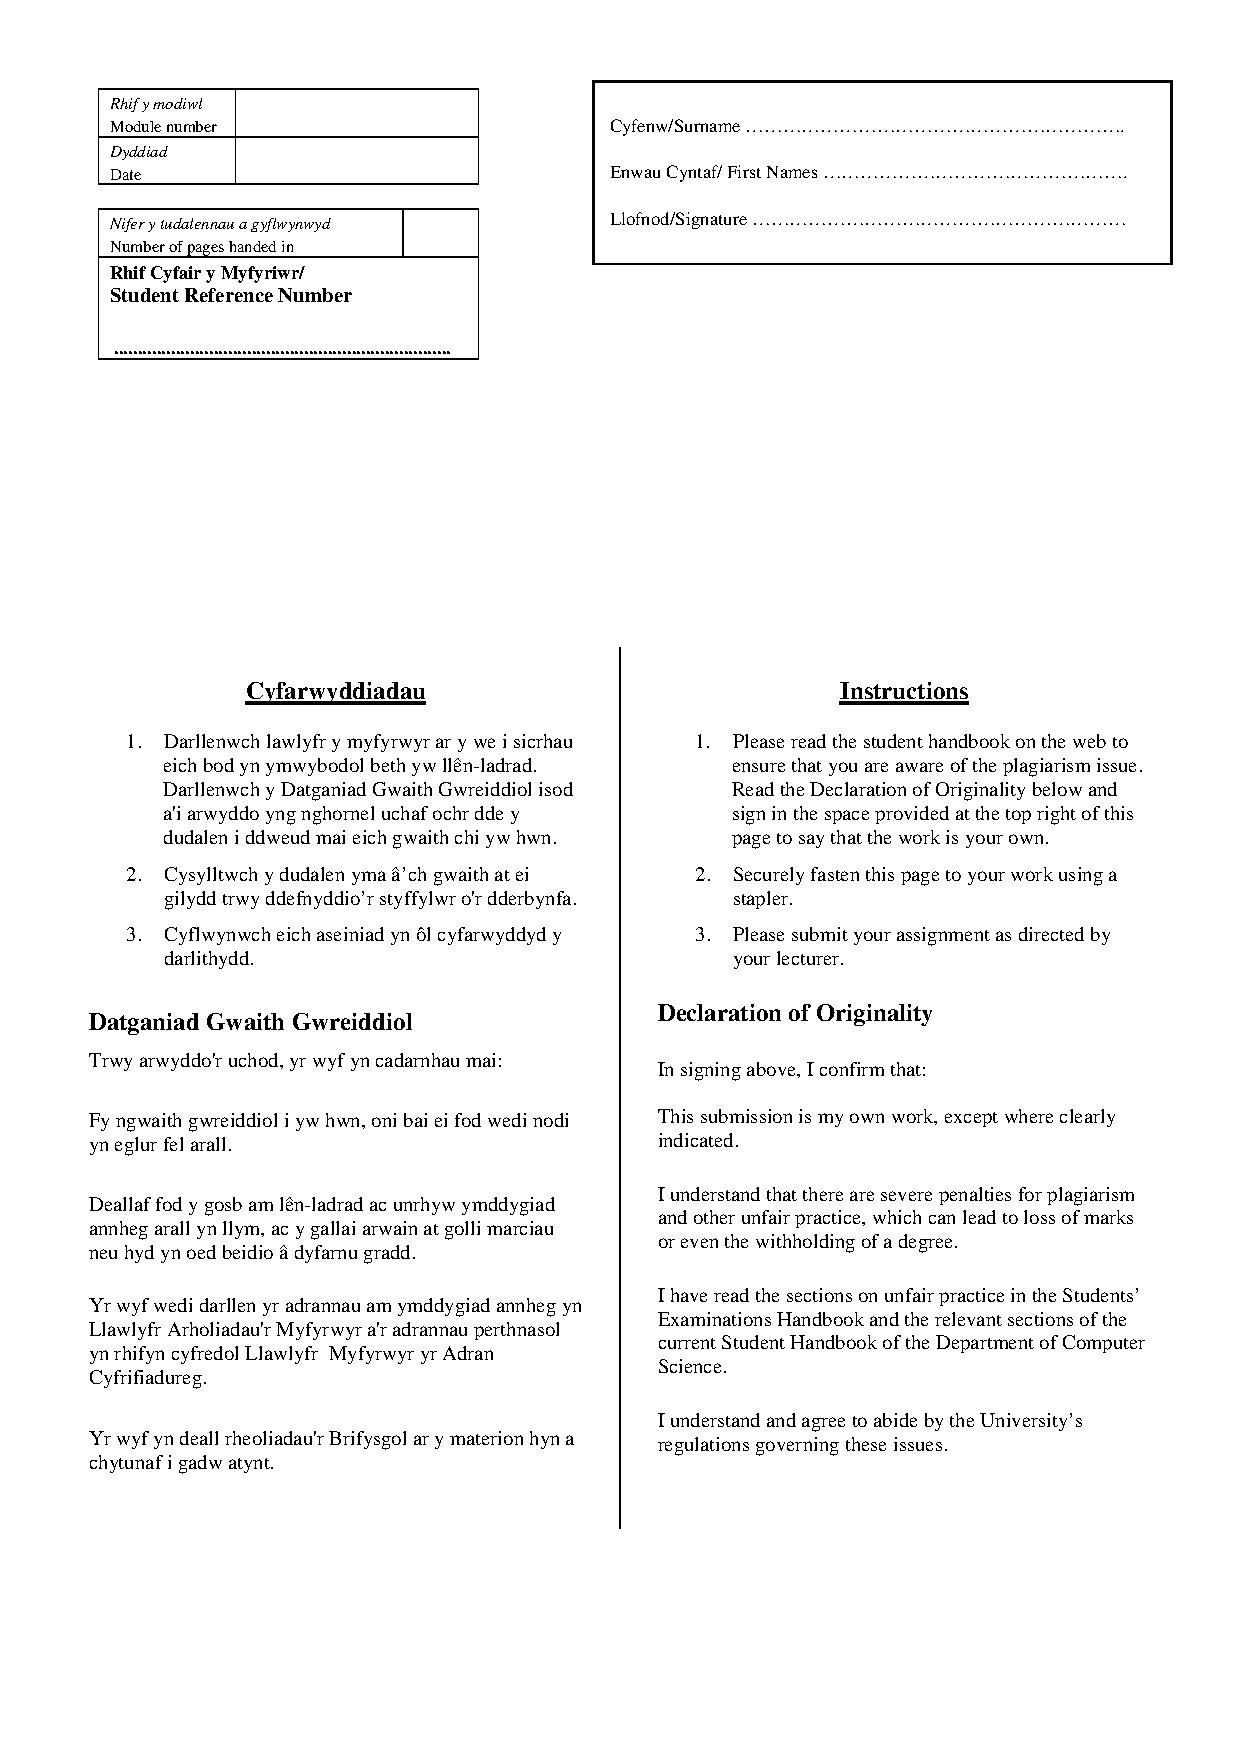
\includepdf{assign_cover.pdf} % Coversheet

\thispagestyle{empty} % Clear page style
\tableofcontents % TOC
\clearpage
\pagenumbering{arabic} % Resets numbering

\section{Introduction}
The purpose of this assignment was to implement a simulated robot to navigate an occupancy grid and then to investigate the differences when this program was used on a real \textit{Pioneer} robot. This involved several aspects including navigation, pathfinding, precision movement, navigation and representation of the (simulated or real) environment using appropriate data structures. 

My implementation focused on the following aspects:

\begin{arrowlist}
    \item{Navigating a simulated grid}
    \item{Searching for an efficient path using data in memory}
    \item{Planning and navigating a given route}
    \item{Versatility in start positions, robot will recalculate its path regularly}
    \item{Environmental awareness of obstacles including disallowing illegal goal positions}
\end{arrowlist}

In addition to this, this program was tested on a real robot and results observed. The pathfinding implementation is deliberative as opposed to reactive - my justification for this is that sonars are unnecessary when a full map of the environment has already been achieved. I familiarised myself with both approaches during the design phase.

Throughout the project, source control was used - both for backup purposes and to provide a record of progress.

\scriptsize
\begin{mdframed}
\verbatiminput{../../Misc/Commit_History.txt}
\end{mdframed}
\normalsize

\section{Player/Stage}
\textit{Player/Stage} is a robotics simulation platform - it combines a simulator (\textit{Stage}) with a client \textit{Player} for use with programming robots. \textit{Player/Stage} makes use of a TCP based architecture \cite{pstcp} and is therefore network aware. With minor changes, the same code used in the simulator can be executed on a real robot.

\textit{Player/Stage} proved difficult to install even on the recommended platform (32-bit Linux) and was prone to crashes and graphical glitches (e.g. grid axis disappearing). I installed it from source on Mac OS X and it was similarly unreliable. Additionally, there was not much documentation provided and the Java API seemed to have a number of bugs. 

For this reason, as well as personal preference, C++ was used to implement my navigation system.
\section{Representation}
The first step to solving the issue of navigating the grid was to determine how best to represent states within the program. I decided to use a \texttt{grid} class to represent the occupancy grid and also need a node class to store potential states for use in a graph search. 
\subsection{Grid Class}
The grid class provides key functionality, it stores the occupancy grid and provides several auxiliary functions to detect 
\subsection{Node Class}
\subsection{Occupancy Grid Mapping}
\begin{lstlisting}
std::pair<int,int> Grid::mapToGridArray(int xPos, int yPos)
{
    std::pair<int,int> arrayPosition;

    arrayPosition.first = 9 - yPos ; // The row
    arrayPosition.second = 10 + xPos; // The column

    return arrayPosition; // Returns the 2D vector indices of the given x,y coordinate
}
\end{lstlisting}
% picture here?
\subsection{Movement}
% discuss booleans
\section{Navigation}
\section{Reactive and Deliberative Pathfinding}
\subsection{Sonar}
\subsection{Graph Search}
\section{Design}
This is design, not error handling.
\subsection{Error Handling}
This is error handling.
\section{Development}
\subsection{Early Ideas}
\subsection{Final Implementation}
\subsection{Future Improvements} % Slightly buggy, more testing, sometimes stops before goal state - if input == currentPos then crash
\section{Testing}
\section{Real Robots}
\section{Conclusions}
\subsection{Evaluation}
\section{References}

%\begin{wrapfigure}{r}{0.5\textwidth}
%    \begin{center}
%            \includegraphics[width=0.47\textwidth]{images/tree.png}
%                \caption{Components of a search tree \hyperref[refs]{[2]}}
%            \end{center}
%        \end{wrapfigure}


%[1] \textit{} [Online]. Available:\\ 
%    \url{}

\end{document}

